% Fig. 1 — architecture overview (draft drawn in TikZ; redraw guide: ../notes/figure_guide.md).
% Colours: carbon@11.84.0 (labdesign build/py/carbon_palette.py). Sensor colours = CATEGORICAL[0..3].
% Thumbnails: figures/fig1_thumbs/ (make with ../figures/src/make_arch_thumbs.py).
% Coordinates in cm; drawing spans x = 0..18.1 (\textwidth = 18.2 cm). Layout rule: every label
% sits at least 1.5 mm inside its box, and no label crosses a line.
\definecolor{cRGB}{HTML}{6929C4}   % cat-1
\definecolor{cDep}{HTML}{1192E8}   % cat-2
\definecolor{cEvt}{HTML}{005D5D}   % cat-3
\definecolor{cLid}{HTML}{9F1853}   % cat-4
\definecolor{acc}{HTML}{0F62FE}    % accent: trained by us
\definecolor{ink}{HTML}{161616}    % fg
\definecolor{mut}{HTML}{525252}    % fg-muted
\definecolor{bd}{HTML}{C6C6C6}     % border
\definecolor{sf}{HTML}{F4F4F4}     % surface
\definecolor{g20}{HTML}{E0E0E0}    % gray-20
\begin{tikzpicture}[
  x=1cm, y=1cm, font=\sffamily\fontsize{6.5}{7.5}\selectfont, line cap=round, line join=round,
  >={Stealth[length=1.6mm, width=1.2mm]},
  flow/.style={->, draw=mut, line width=0.45pt},
  tflow/.style={->, draw=acc, line width=0.6pt},
  frozen/.style={draw=mut, dash pattern=on 1.6pt off 1.2pt, line width=0.45pt, fill=sf},
  trained/.style={draw=acc, line width=0.7pt, fill=white},
  plain/.style={draw=mut, line width=0.45pt, fill=white},
  ttl/.style={font=\sffamily\bfseries\fontsize{6.8}{8}\selectfont, text=ink},
  sub/.style={text=mut, font=\sffamily\fontsize{5.6}{6.6}\selectfont},
  plab/.style={font=\sffamily\bfseries\fontsize{8}{9}\selectfont, text=ink, anchor=west},
  plus/.style={circle, inner sep=0pt, minimum size=2.6mm, fill=white},
]
% ======================= (a) inference =======================
\node[plab] at (0.0,6.75) {(a)};
\node[ttl, anchor=west] at (0.5,6.75) {Inference: one frozen backbone, sensor-specific adapters, cross-modal fusion};

% --- sensor thumbnails ---
\foreach \s/\f/\c/\yy in {RGB/rgb/cRGB/5.15, Depth/depth/cDep/3.9, Event/event/cEvt/2.65, LiDAR/lidar/cLid/1.4}{
  \node[inner sep=0pt] (in\s) at (0.9,\yy) {\includegraphics[width=1.05cm]{figures/fig1_thumbs/\f.png}};
  \draw[\c, line width=0.9pt] (in\s.south west) rectangle (in\s.north east);
  \node[anchor=south, rotate=90, text=\c, font=\sffamily\bfseries\fontsize{6}{7}\selectfont, inner sep=2pt] at (in\s.west) {\s};
}

% --- frozen backbone, one lane per sensor ---
\draw[frozen, rounded corners=1.5pt] (1.8,0.85) rectangle (5.0,6.15);
\node[ttl, anchor=north west] at (1.92,6.02) {DINOv3-L};
\node[sub, anchor=north east] at (4.88,6.0) {frozen, shared};
\node[sub, anchor=east] at (2.62,5.52) {tap};
\foreach \t/\xx in {6/3.25, 12/3.77, 18/4.29, 24/4.81}{ \node[sub] at (\xx,5.52) {\t}; }
\foreach \s/\c/\yy in {RGB/cRGB/5.15, Depth/cDep/3.9, Event/cEvt/2.65, LiDAR/cLid/1.4}{
  \draw[draw=\c, fill=\c!14, line width=0.6pt, rounded corners=0.8pt] (1.97,\yy-0.19) rectangle (2.62,\yy+0.19);
  \node[text=\c, font=\sffamily\bfseries\fontsize{5.2}{6}\selectfont, inner sep=0pt] at (2.295,\yy) {LoRA};
  \foreach \k in {0,...,3}{
    \draw[draw=bd, fill=g20, line width=0.35pt] (2.82+0.52*\k,\yy-0.16) rectangle (3.18+0.52*\k,\yy+0.16);
    \fill[\c] (3.25+0.52*\k,\yy) circle (0.045);
  }
  \draw[flow] (in\s.east) -- (1.97,\yy);
}

% --- per-sensor token sets ---
\node[sub] at (5.5,6.0) {tokens};
\foreach \s/\c/\yy in {RGB/cRGB/5.15, Depth/cDep/3.9, Event/cEvt/2.65, LiDAR/cLid/1.4}{
  \foreach \k in {3,2,1,0}{
    \draw[draw=\c, fill=\c!20, line width=0.4pt] (5.25+0.06*\k,\yy-0.17+0.06*\k) rectangle +(0.3,0.3);
  }
  \coordinate (tok\s) at (5.8,\yy+0.05);
}

% --- cross-modal attention (trained) ---
\draw[trained, rounded corners=1.5pt] (6.2,1.3) rectangle (8.4,5.65);
\node[ttl, align=center] at (7.3,5.12) {Cross-modal\\attention};
\coordinate (K) at (7.3,3.55);
\foreach \s/\a in {RGB/135, Depth/45, Event/-45, LiDAR/-135}{ \coordinate (n\s) at ($(K)+(\a:0.68)$); }
\foreach \p/\q in {RGB/Depth, RGB/Event, RGB/LiDAR, Depth/Event, Depth/LiDAR, Event/LiDAR}{
  \draw[<->, draw=mut!70, line width=0.4pt, >={Stealth[length=1.1mm,width=0.9mm]}, shorten <=1.5mm, shorten >=1.5mm] (n\p) -- (n\q);
}
\foreach \s/\c in {RGB/cRGB, Depth/cDep, Event/cEvt, LiDAR/cLid}{ \fill[\c] (n\s) circle (0.1); }
\node[sub, align=center] at (7.3,1.9) {each sensor attends\\to the other sensors\\2 layers};
\foreach \s/\yy in {RGB/4.85, Depth/3.95, Event/3.05, LiDAR/2.2}{
  \draw[flow] (tok\s) to[out=0, in=180] (6.2,\yy);
}

% --- SimpleFPN (conventional) ---
\draw[plain, draw=bd, rounded corners=1.5pt] (8.68,1.7) rectangle (10.15,5.65);
\node[ttl] at (9.45,5.38) {SimpleFPN};
\foreach \lab/\w/\yy in {{1/32}/0.32/4.75, {1/16}/0.44/4.05, {1/8}/0.58/3.2, {1/4}/0.76/2.2}{
  \draw[plain] (9.6-\w/2,\yy-\w/2) rectangle (9.6+\w/2,\yy+\w/2);
  \node[sub, anchor=east] at (9.6-\w/2-0.06,\yy) {\lab};
}
\draw[flow] (8.4,3.2) -- (8.68,3.2);
\node[plus, draw=mut, line width=0.45pt] (sum) at (9.6,1.05) {};
\draw[mut, line width=0.45pt] (sum.north) -- (sum.south) (sum.west) -- (sum.east);
\draw[flow] (sum) -- (9.6,1.82);
\node[sub, anchor=west] at (9.78,1.05) {sum per level};

% --- high-resolution path (adopted from the DINOv3 adapter) ---
\draw[flow] (inLiDAR.south) -- (0.9,0.35) -- (2.05,0.35);
\node[sub, anchor=north] at (1.47,0.3) {full-res. input};
\draw[plain, rounded corners=1.2pt] (2.05,0.12) rectangle (3.45,0.58);
\node[text=ink] at (2.75,0.35) {conv stem};
\draw[flow] (3.45,0.35) -- (3.8,0.35);
\draw[plain, rounded corners=1.2pt] (3.8,0.12) rectangle (6.75,0.58);
\node[text=ink] at (5.275,0.35) {deformable extractors ($\times$6)};
\draw[->, draw=mut, line width=0.45pt, dash pattern=on 1.4pt off 1pt] (4.35,0.85) -- (4.35,0.58);
\node[sub, anchor=west] at (4.42,0.72) {samples tap tokens};
\draw[flow] (6.75,0.35) -| (sum.south);
\node[sub, anchor=south] at (8.1,0.38) {high-resolution path};

% --- heads (trained) ---
\draw[flow] (10.15,3.2) -- (10.3,3.2) |- (10.5,4.75);
\draw[flow] (10.3,3.35) -- (10.5,3.35);
\draw[trained, rounded corners=1.2pt] (10.5,4.4) rectangle (11.95,5.1);
\node[ttl] at (11.225,4.87) {Dense head};
\node[sub] at (11.225,4.6) {per-pixel};
\draw[trained, rounded corners=1.2pt] (10.5,2.75) rectangle (11.95,3.95);
\node[ttl] at (11.225,3.7) {Query head};
\foreach \k in {0,...,7}{ \fill[acc!55] (10.805+0.12*\k,3.36) circle (0.035); }
\node[sub] at (11.225,3.03) {100 queries};
\node[plus, draw=acc, line width=0.6pt] (arb) at (12.35,3.35) {};
\draw[acc, line width=0.6pt] (arb.north) -- (arb.south) (arb.west) -- (arb.east);
\draw[tflow] (11.95,4.75) -| (12.75,3.35) -- (arb.east);
\draw[tflow] (11.95,3.35) -- (arb.west);
\node[sub, anchor=north west] at (12.45,3.2) {arbiter};
\node[inner sep=0pt] (pred) at (12.35,1.45) {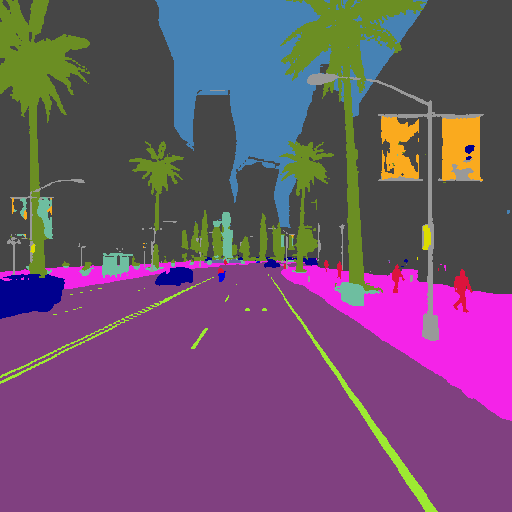
\includegraphics[width=1.05cm]{figures/fig1_thumbs/pred.png}};
\draw[ink, line width=0.5pt] (pred.south west) rectangle (pred.north east);
\draw[tflow] (arb.south) -- (pred.north);
\node[sub, anchor=north] at (pred.south) {prediction};

% ======================= (b) training =======================
\draw[bd, line width=0.4pt] (13.2,0.05) -- (13.2,6.6);
\node[plab] at (13.35,6.75) {(b)};
\node[ttl, anchor=west] at (13.85,6.75) {Training: clean and degraded passes};

\node[inner sep=0pt] (cl) at (14.1,4.9) {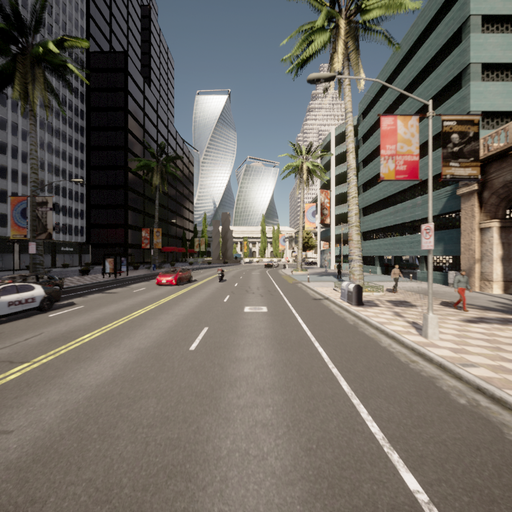
\includegraphics[width=0.95cm]{figures/fig1_thumbs/rgb.png}};
\node[sub, anchor=north] at (cl.south) {clean};
% degraded RGB in front of a dropped sensor
\draw[draw=mut, fill=white, line width=0.4pt] (14.1-0.475+0.15,2.8-0.475-0.15) rectangle (14.1+0.475+0.15,2.8+0.475-0.15);
\draw[mut, line width=0.35pt] (14.1-0.475+0.15,2.8-0.475-0.15) -- (14.1+0.475+0.15,2.8+0.475-0.15);
\node[inner sep=0pt] (dg) at (14.1,2.8) {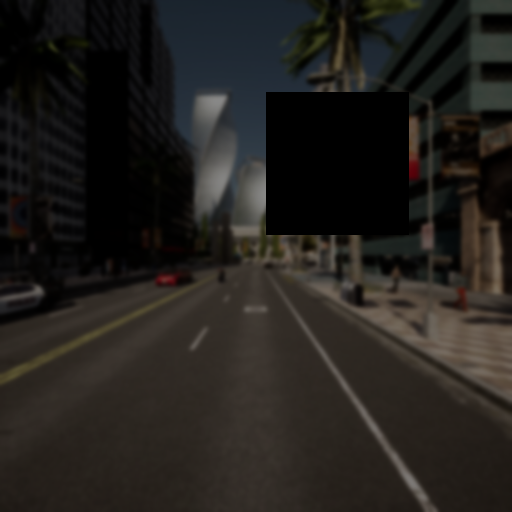
\includegraphics[width=0.95cm]{figures/fig1_thumbs/rgb_degraded.png}};
\node[sub, anchor=north, align=center] at (14.2,2.12) {degraded\\(blur, exposure,\\sensor dropout)};

\draw[trained, rounded corners=1.5pt] (14.95,2.3) rectangle (16.45,5.4);
\node[ttl] at (15.7,4.05) {Model (a)};
\node[sub, align=center] at (15.7,3.62) {same\\weights};
\draw[flow] (cl.east) -- (14.95,4.9);
\draw[flow] (dg.east) ++(0.15,0) -- (14.95,2.8);

\draw[frozen, rounded corners=1.5pt] (14.95,0.3) rectangle (16.45,1.5);
\node[ttl] at (15.7,1.2) {Teacher};
\node[sub, align=center] at (15.7,0.77) {frozen,\\clean-trained};
\draw[flow] (cl.west) -- (13.38,4.9) |- (14.95,0.9);

\node[anchor=west, text=ink, inner sep=1pt] (ce1) at (16.85,4.9) {$\mathcal{L}_{\mathrm{CE}}$};
\node[anchor=west, text=ink, inner sep=1pt] (ce2) at (16.85,3.2) {$\mathcal{L}_{\mathrm{CE}}$};
\node[anchor=west, text=acc, inner sep=1pt] (kd) at (16.85,2.4) {$\mathcal{L}_{\mathrm{KD}}$};
\draw[flow] (16.45,4.9) -- (ce1.west);
\draw[flow] (16.45,2.8) -- (16.65,2.8) |- (ce2.west);
\draw[flow] (16.65,2.8) |- (kd.west);
\draw[->, draw=acc, line width=0.55pt, dash pattern=on 1.4pt off 1pt] (16.45,0.9) -| (kd.south);
\node[sub, anchor=west, align=left] at (17.25,1.3) {soft\\targets\\$T{=}2$};
\end{tikzpicture}
